\documentclass[11pt]{article}

\usepackage{epsfig,amsmath,amssymb,amsfonts,amstext,amsthm,enumerate}
\usepackage{latexsym,graphics,epsf,epsfig,color}
\usepackage{cite,url}
\usepackage{graphicx}

\textwidth 6.65in \oddsidemargin -0.1in \topmargin -0.5in
\textheight 8.8in

\newtheorem{theorem}{Theorem}
\newtheorem{prop}{Proposition}
\newtheorem{lemma}{Lemma}
%\newtheorem{coro}[theorem]{Corollary}
\newtheorem{coro}{Corollary}
\newtheorem{defi}{Definition}
\newtheorem{algo}{Algorithm}
\newtheorem{remark}{Remark}
\newtheorem{fact}{Fact}
\newtheorem{claim}{Claim}

\newcommand{\defeq}[1]{\;{\buildrel\rm{#1}\over=}\;}
\newcommand{\defleq}[1]{\;{\buildrel\rm{#1}\over\leq}\;}
\newcommand{\defgeq}[1]{\;{\buildrel\rm{#1}\over\geq}\;}
\newcommand{\scite}[1]{\textsuperscript{\cite{#1}}} %????????


%\linespread{1.6667}
\usepackage{setspace}
%\doublespacing
\begin{document}


\title{Modification to CATS by assigning adaptive weights to the parameters by assessing how spammers evolve through the network}

\author{ Ravi Sankar Raju, Xinyi Cai}


\date{\today}

\maketitle

\begin{abstract}
With the advent of social networking, online media has gained a lot of popularity. To the extent that mainstream media has taken a backseat. People like to have instant updates on things and people that interest them. In this regard, social media are, in a way a tailor made electronic newspaper that people have access to round the clock. Twitter with its microblogging feature, is even more efficient in delivering news in a crisp and concise fashion. But, as with any technology, twitter too can be used in negative ways. One of the most common ways to exploit twitter is spam. Spammers propagate falsified information hidden behind an shortened URL, luring the users to open the web pages. These web pages might either have some irrelevant advertisements or might be a security threat which affects the user's system without his notice. One of the most common ways to get the users to click the URLs are by using trending topics. This research work identifies characteristics of such spammers that can be used to identify them in the twitter. Ground truth is used to train a classifier which is then validated in two different ways. There's a high percentage of accuracy with the detection, around 99. Also, the most important attributes that contribute to the the decision making are discussed.
\end{abstract}

\section{Introduction and Prior Works}

With the size of twitter and its user base its almost inevitable to have a spam free environment. And spam is not just a false marketing or a virus attack. Things like profanity, insults, hate speech, fraudulent reviews, fake profiles constitutes a little part of an exhaustive list, if there exists one. Why twitter ? Twitter is more easy to spam because of its microblogging facility. If you can get people interested in 140 characters, then you can get them to click a link or buy a product even. As they say, curiosity kills. Any other social media has a larger content disposition which tends to give the user more than what is necessary and hence sometime reveals the trick.
Effects of spam in twitter is not only realized by the end users. Imagine the amount of useless data twitter has to store, process and maintain. Its a waste of resource and time from twitter's perspective. Detection of Spammers is not so easy after all. Although twitter has become better at eliminating spammers recently, still there are a lot of spammers that are hiding perfectly. This is becase spammers evolve along with the spam detection strategies.

Trending tags are a major way in which spam propogates through the network. An instance of this would be using tags like "blackfriday" and "cybermonday" during thanksgiving time. More people are likely to be searching for deals and this gives an edge to spammers who can use this tag and lure an user into doing something that they wouldn't normally do. If an ad says "iPad for 100\$, hurry up! goo.gl/sX7gIV", people would normally open the link. More than 99\% of the internet users will not know the implications of hitting a bad URL. This can be detected and eliminated only to an extent, partly due to the high volume of tweets that flows through the network during this time.

There has been a lot of works going on recently to detect spammers. Some of them are "Detecting Spammers on Twitter" by F. Benevenuto and G. Magno's work$^{[1]}$, "CATS: Characterizing Automation of Twitter Spammers" by A. Amleshwaram and N. Reddy's paper$^{[2]}$. The former one defines a set of 62 characteristics with which they train a classifier to detect spammers. The latter one differs in the types of characteristics in addition to understanding spam campaigns.

Our work can be split as,
\begin{enumerate}
\item Collection of Data. Ground Truth has been obtained from "http://homepages.dcc.ufmg.br/~fabricio/spammerscollection.html", the author of the first paper. Similarly Ground truth for Non Spammers are collected. Lastly, users who tweeted about trending topics are identified as a test set.
\item Constructing the Classifier. Using weka, an opensource tool for machine learning, a classifier is generated from the groundtruth.
\item Analysis of the features. Out of the 58 features (we use only 58 of the 62), we analyse what features are more important in the decision making process.
\end{enumerate}
%problem statement and main work
\section{Background and Dataset Collection}
\subsection{Background}
Twitter is a social network where you can follow other persons to get their updates(tweets). Anyone can be followed from a friend to a rockstar, provided they are in the system. It also serves as a great source of news to a lot of people who seek news in twitter. Tweets are posts that are limited in length to 140 characters. You can reply to a tweet or retweet, which is basically sharing. Also you can tag another person while tweeting. This is called mentioning in twitter terminology. The \# symbol followed by a word, called a hashtag, is used to mark  topics in a Tweet. The hashtags play a major role in identifying current trends.

\subsection{About the API}
Twitter provides an API to tap into his data for research and other purposes. To use the API, one has to be registered in dev.twitter.com and have a valid twitter account. Tweepy is the python library that we have used in this project to get data from twitter. Twitter exposes about 1\% of its data to the API, and the API has a rate limiting. There is a limit of 15 requests per 15 minutes. Almost all requests are rate limited. Because of this it is a timetaking process to collect data from twitter. For instance if you are trying to collect the follower list of a public figure who has 100000 followers, it is going to take 500 requests (each request allows a maximum of 200 tuples). Hence it gets difficult. This is the reason why only 58 features has been used from the dataset. With more time, it is possible to analyse such huge volumes of data. There's a streaming API which gets the current tweets across the world.

\subsection{Data Collection}
%build dataset of a number of random users
The Dataset of Ground truth has two parts. Spammers and Non Spammers. The former is obtained from the author of "Detection of Spammers in Twitter" \scite{1}. For Non spammers, we collect the followers and following of my own account which I manually know to be genuine, a total of 469 users. 58 features that are mentioned below in the report has been extracted for each of these users. 

The current trends at the time of tweet collection were 'Thanksgiving', 'TellyExpressFaceOfTheYear', 'ThanksToStarWars', 'MomInspirations', 'tejpal', 'Jordan Hill', 'GarthBrooks'. Tweets from the streaming API were obtained, filtered on these terms and saved in JSON format. Unique user obejcts were collected from these tweets and the feature set is extracted for them as well. This will serve as one of the test set. Other test set would be a random percentage of the ground truth which is not used for building the classifier. Hence if 60\% is the limit, then only 60\% of the ground truth will be used in construction of the data set. The rest 40\% is used as a test set. 

\section{Twitter users' features and Main Result}
% evaluate 58 users feature and result comparison of spammers and non-spammers, the result applied to detect spammers
We evaluate 58 features of the pre-classified dataset of spammers and non-spammer users. The 58 features would be divided into two category: content attributes and user behavior attributes. Content attributes are properties of the text of tweets posted by users, which capture specific properties related to the way users write tweets. User behavior attributes capture specific properties of the user behavior in terms of the posting frequency, social interactions, and influence on the Twitter network. 
\subsection{Content Attributes}
  In total, we have 37 attributes related to content of the tweets. That is, number of URLs in each tweet, number of hashtags, number of words on each tweet, number of users mentioned in each tweet, number of character, count of numbers and so on. The list of attributes can be found in the appendix
\subsection{User behavior Attributes}
 In total, we have 21 attributes about the user behavior. As assumed and according to the measurement of our dataset, spammers are more likely to have less followers, more followees, lower number of times the user was mentioned, lower number of times the user was replied to, lower number of times the user replied someone, lower number of followees of the users followers (since they are more likely to be spammers as well), more fixed time between tweets, and more fixed tweets posted per day and per week.


\section{Detecting Spammers}

In this section we go about how we train the classifier with our ground truth and how we use it to detect spammers. There are two different testing strategies which will be discussed. Also, the effectiveness of the features will be analysed from the decision tree constructed to classify. Finally we talk about metrics such as correctness and false positive results.

\subsection{Building and Training the Classifier}
We use weka (waikato environment for knowledge analysis), an opensource machine learning tool. The input data is converted into .arff format and feeded into the system. J48 classifier is constructed, which classifies the instance 99.217\% correctly. The confusion matrix is

\begin{table}[ht] 
\caption{Classifier Confusion Matrix} % title of Table 
\centering % used for centering table 
\begin{tabular}{c c c c} % centered columns (4 columns) 
\hline\hline %inserts double horizontal lines 
Case & spammer & non spammer & classified as \\ [0.5ex] % inserts table 
%heading 
\hline % inserts single horizontal line 
1 & 1056 & 9 & spammer \\ % inserting body of the table 
2 & 3 & 466 & non spammer \\ [1ex] % [1ex] adds vertical space 
\hline %inserts single line 
\end{tabular} 
\label{table:nonlin} % is used to refer this table in the text 
\end{table}

The table shows that 1056 out 1065 spammers has been represented correctly by the classifier. Similarly, 466 out of the 469 real users fit into the system. A total of 12 users are found as outliers. 99.22\% is a good correctness for a classifier. The classifier tries to find mean and median for each of the 58 features, and then picks up features in order of decreasing solvability. solvability of a feature is defined as how well it can delineate the dataset into different paths so that the decision tree is minimum. If we take all possible paths the tree would be have a depth of P(58,2). Few examples of how each feature separates the ground truth can be viewed from the Figure 1 and Figure 2. Blue is Spammer, which remains predominantly at the bottom half of the feature range for most of the featrues, while red, the non spammer have higher values in most of the cases.

\begin{figure}
\centering
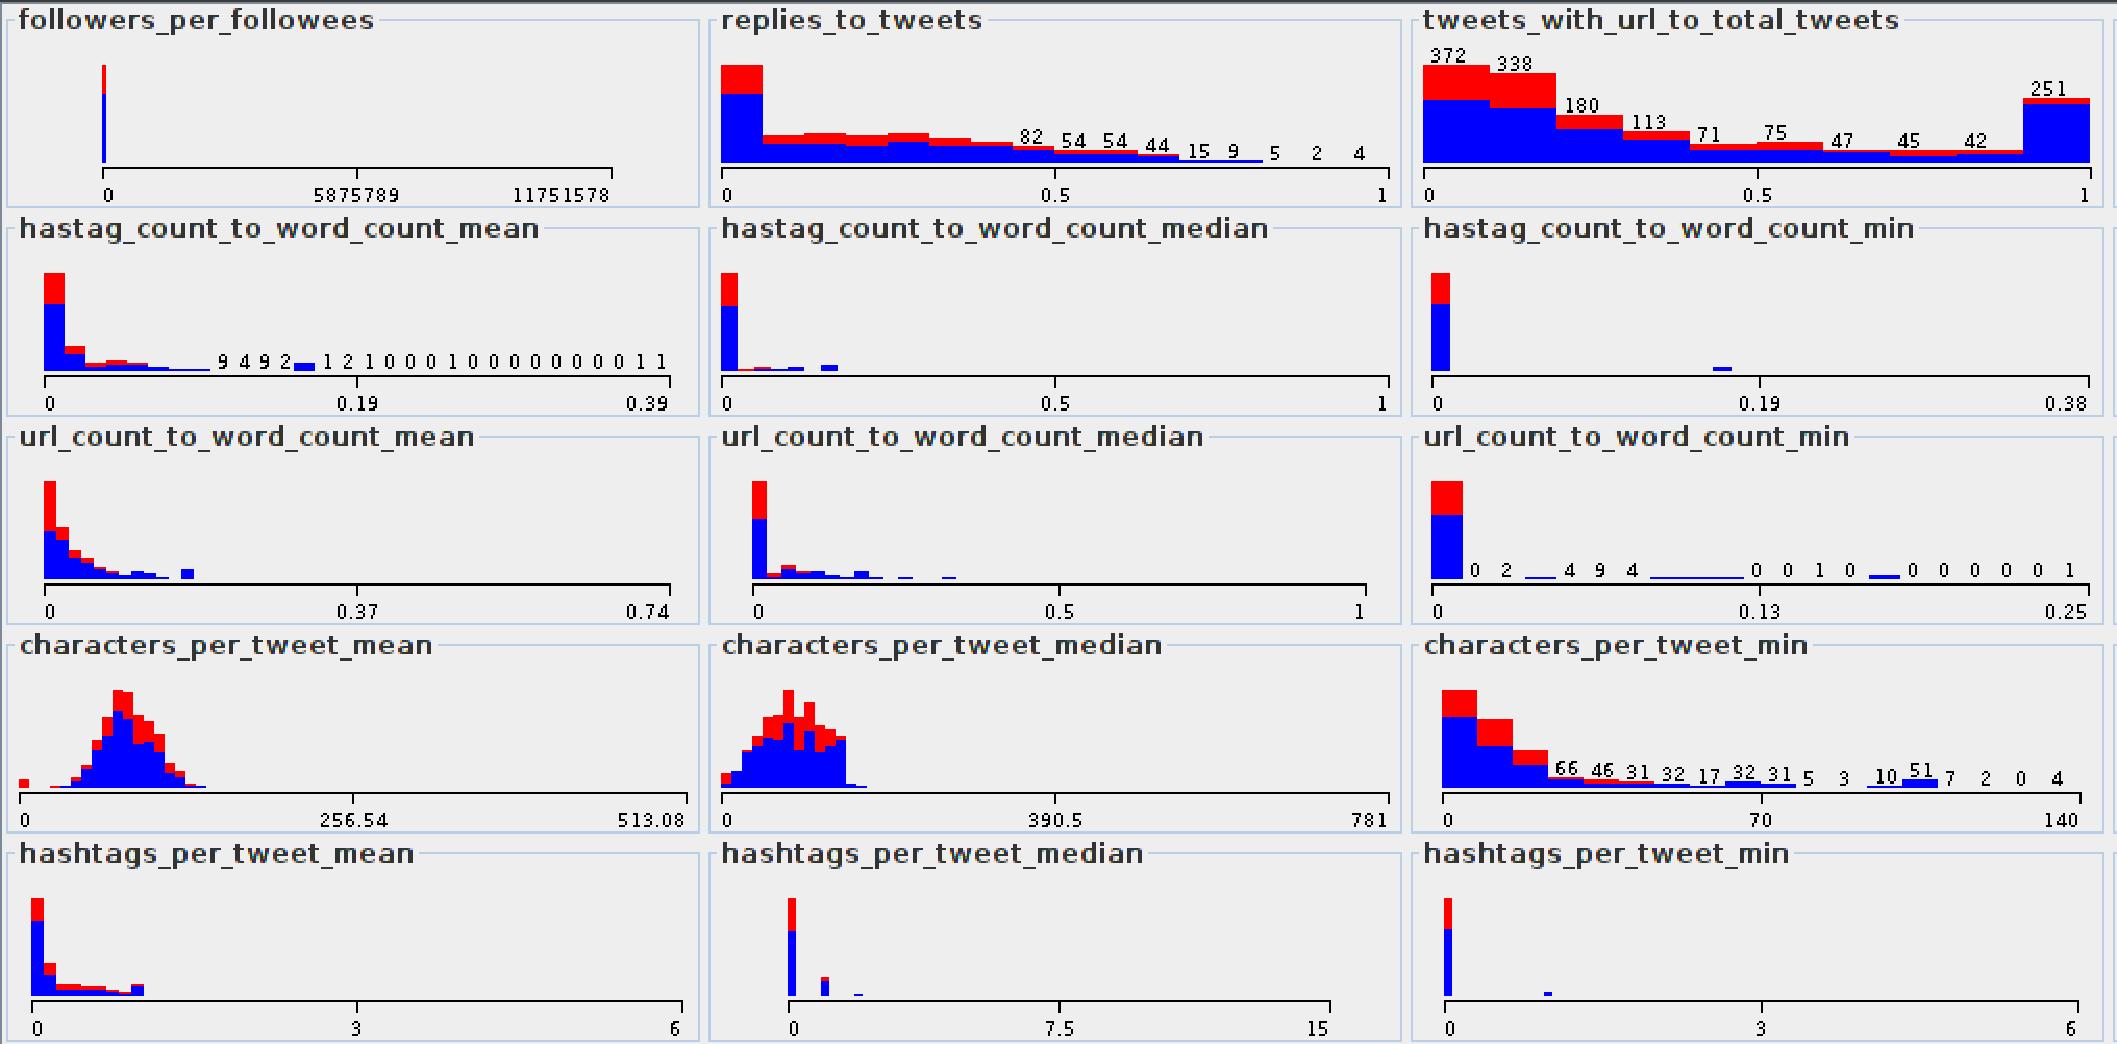
\includegraphics[width=0.80\textwidth,natwidth=610,natheight=642]{feature_vs_spammer_class_1.pdf}
\caption{Feature vs Spammer Class}
\end{figure}

\begin{figure}
\centering
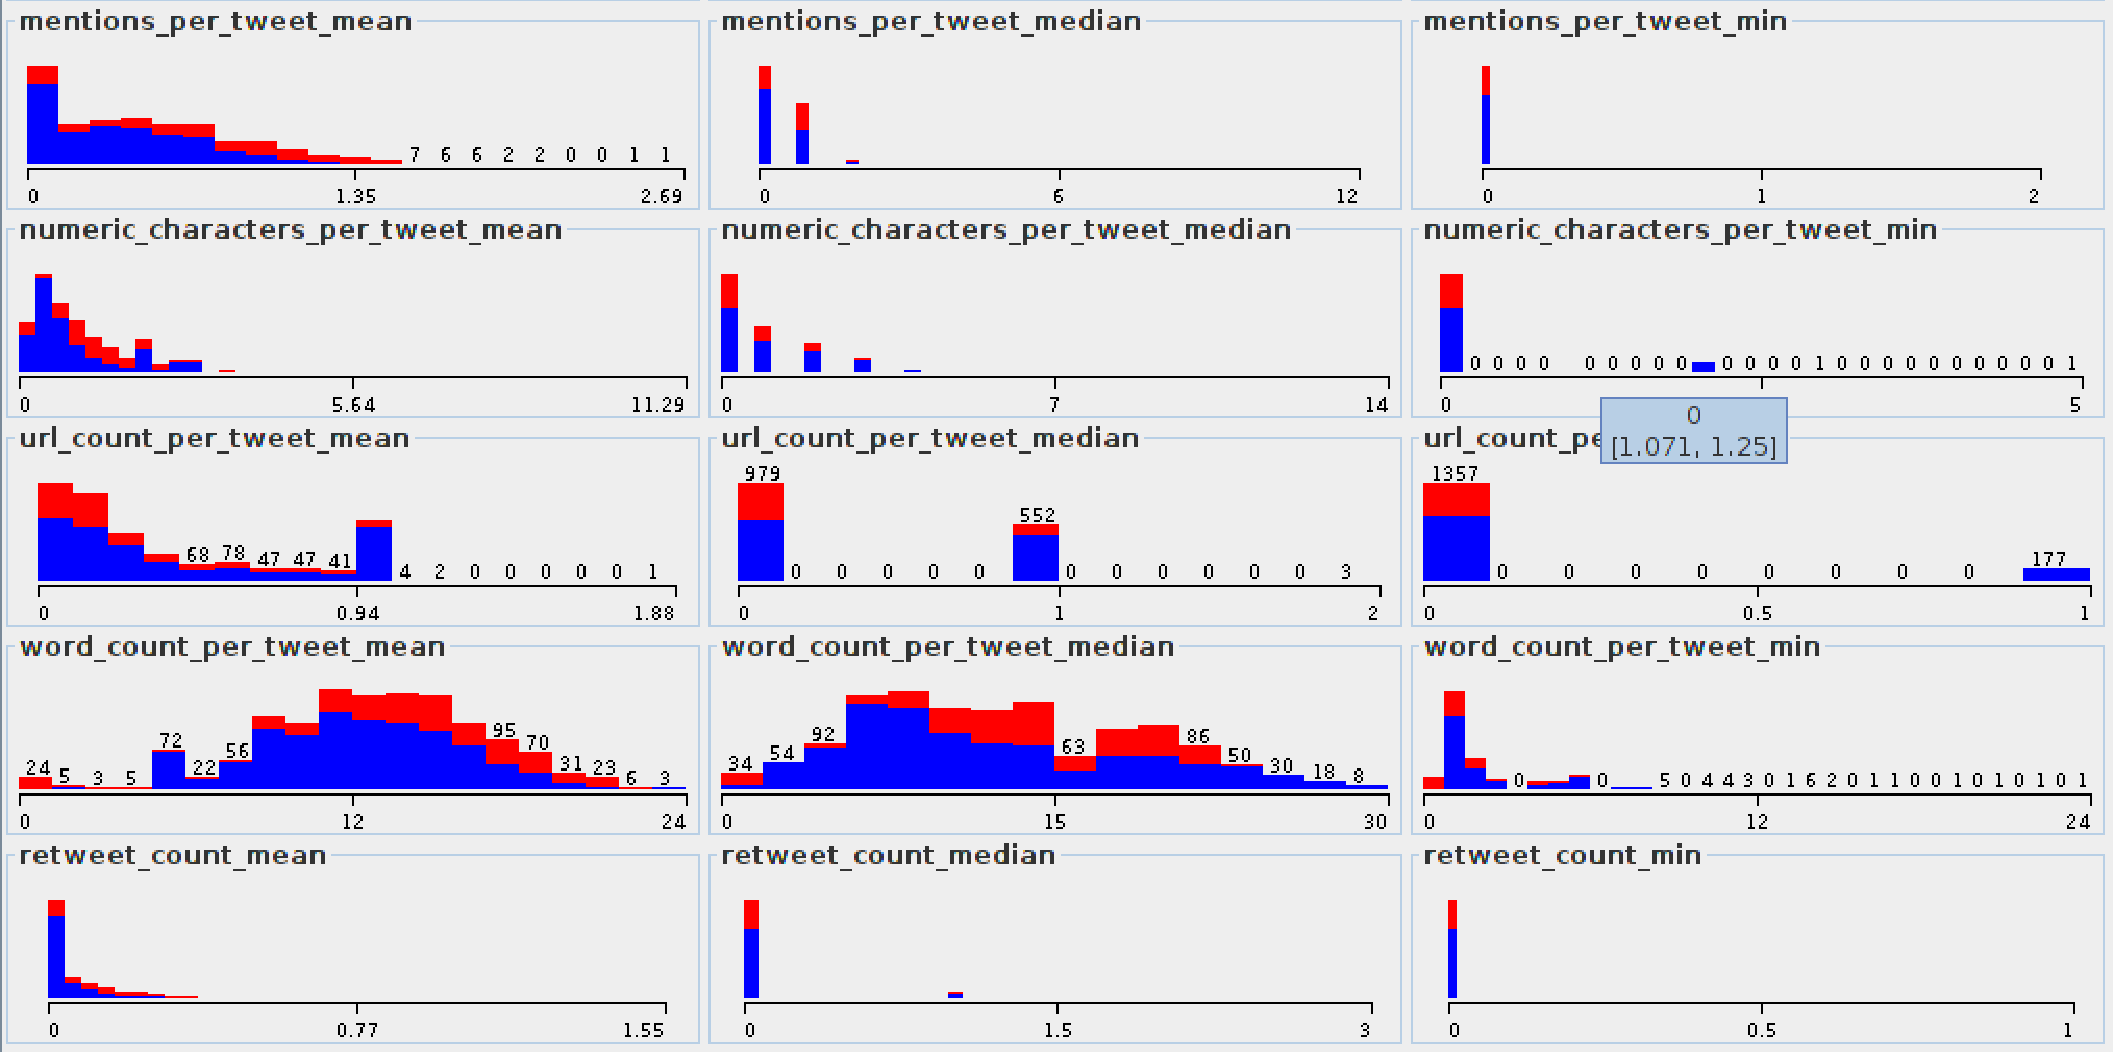
\includegraphics[width=0.80\textwidth,natwidth=610,natheight=642]{feature_vs_spammer_class_2.pdf}
\caption{Feature vs Spammer Class}
\end{figure}

\subsection {Results and Observations}
Now there are two ways to test the classifier.
\begin{enumerate}
\item Introducing new test set. The new training set is obtained by observing the tweets from the Twitter Streaming API and filtering them on the latest trends. Using this tweet details 30 users were chose and their features were extracted. 30 more users from a pre recognized spam list was added to this test set. This pre recognized list was obtained from internet (http://www.infochimps.com/datasets/twitter-spammers-list). This feature set was converted into .arff file format and fed into the J48 classifier and the results were as follows. While feeding, it was assumed that none of the spammers so that we will know what the classifier thinks. It turns out that 59 out of the 60 users are non spammers and one user was a spammer. The output of the classifier is shown in the Table.

\begin{table}[ht] 
\caption{Classifier Confusion Matrix for the Test set} % title of Table 
\centering % used for centering table 
\begin{tabular}{c c c c} % centered columns (4 columns) 
\hline\hline %inserts double horizontal lines 
Case & spammer & non spammer & classified as \\ [0.5ex] % inserts table 
%heading 
\hline % inserts single horizontal line 
1 & 0 & 0 & spammer \\ % inserting body of the table 
2 & 1 & 59 & non spammer \\ [1ex] % [1ex] adds vertical space 
\hline %inserts single line 
\end{tabular} 
\label{table:nonlin} % is used to refer this table in the text 
\end{table}

The expected result though should have been 30 spammers and 30 non spammers. We are unfortunate to not be able to know for sure if the result was correct. But when we looked at the one account that was reported to be a spammer, it was pretty inactive and did not look like a spammer at all. There's a high chance that there were no spammers in the set of 30 users obtained from the streaming API. 30 is a pretty small value if you consider the number of user twitter has. However, the other 30 of the the 60 users are supposed to be spammers. But it turned out that the names found as spammers in the web provided list did not look like spammers either, when we tried to verify them manually. It could also be that, the classifier is not good enough to capture the latest trends in evolution of spammers. Hence, we test the classifier in another way. Also, a better way to get spammer test data is discussed later in the paper.

\item Using a part of the groundtruth. weka provides a test option called percentage split, where only a given percentage of groundtruth is used for the construction of classifier. The remaning part of the data is used to test the classifier. The part of the data is selected randomly for each run. This method was run for 10\%, 50\%, 66\% and the results are shown in the table. The percentage of accuracy is 94.7864\%,  99.3481\%, 99.6169\% respectively


\begin{table}[ht] 
\caption{Classifier Confusion Matrix for the Test set at 10\%} % title of Table 
\centering % used for centering table 
\begin{tabular}{c c c c} % centered columns (4 columns) 
\hline\hline %inserts double horizontal lines 
Case & spammer & non spammer & classified as \\ [0.5ex] % inserts table 
%heading 
\hline % inserts single horizontal line 
1 & 926 & 39 & spammer \\ % inserting body of the table 
2 & 33 & 383 & non spammer \\ [1ex] % [1ex] adds vertical space 
\hline %inserts single line 
\end{tabular} 
\label{table:nonlin} % is used to refer this table in the text 
\end{table}


\begin{table}[ht] 
\caption{Classifier Confusion Matrix for the Test set at 50\%} % title of Table 
\centering % used for centering table 
\begin{tabular}{c c c c} % centered columns (4 columns) 
\hline\hline %inserts double horizontal lines 
Case & spammer & non spammer & classified as \\ [0.5ex] % inserts table 
%heading 
\hline % inserts single horizontal line 
1 & 539 & 3 & spammer \\ % inserting body of the table 
2 & 2 & 223 & non spammer \\ [1ex] % [1ex] adds vertical space 
\hline %inserts single line 
\end{tabular} 
\label{table:nonlin} % is used to refer this table in the text 
\end{table}

\begin{table}[ht] 
\caption{Classifier Confusion Matrix for the Test set at 66\%} % title of Table 
\centering % used for centering table 
\begin{tabular}{c c c c} % centered columns (4 columns) 
\hline\hline %inserts double horizontal lines 
Case & spammer & non spammer & classified as \\ [0.5ex] % inserts table 
%heading 
\hline % inserts single horizontal line 
1 & 371 & 2 & spammer \\ % inserting body of the table 
2 & 0 & 149 & non spammer \\ [1ex] % [1ex] adds vertical space 
\hline %inserts single line 
\end{tabular} 
\label{table:nonlin} % is used to refer this table in the text 
\end{table}

The observation from the these values and from the table is that the data from ground truth is quite consistent and there are less abnormalities. That's why even a classifier trained with as less at 10\% of data is able to give startling results. Atleast the classifier works correctly. 
\end{enumerate}

\subsection{Analysis of the Decision Tree and the Features}
\begin{figure}
\centering
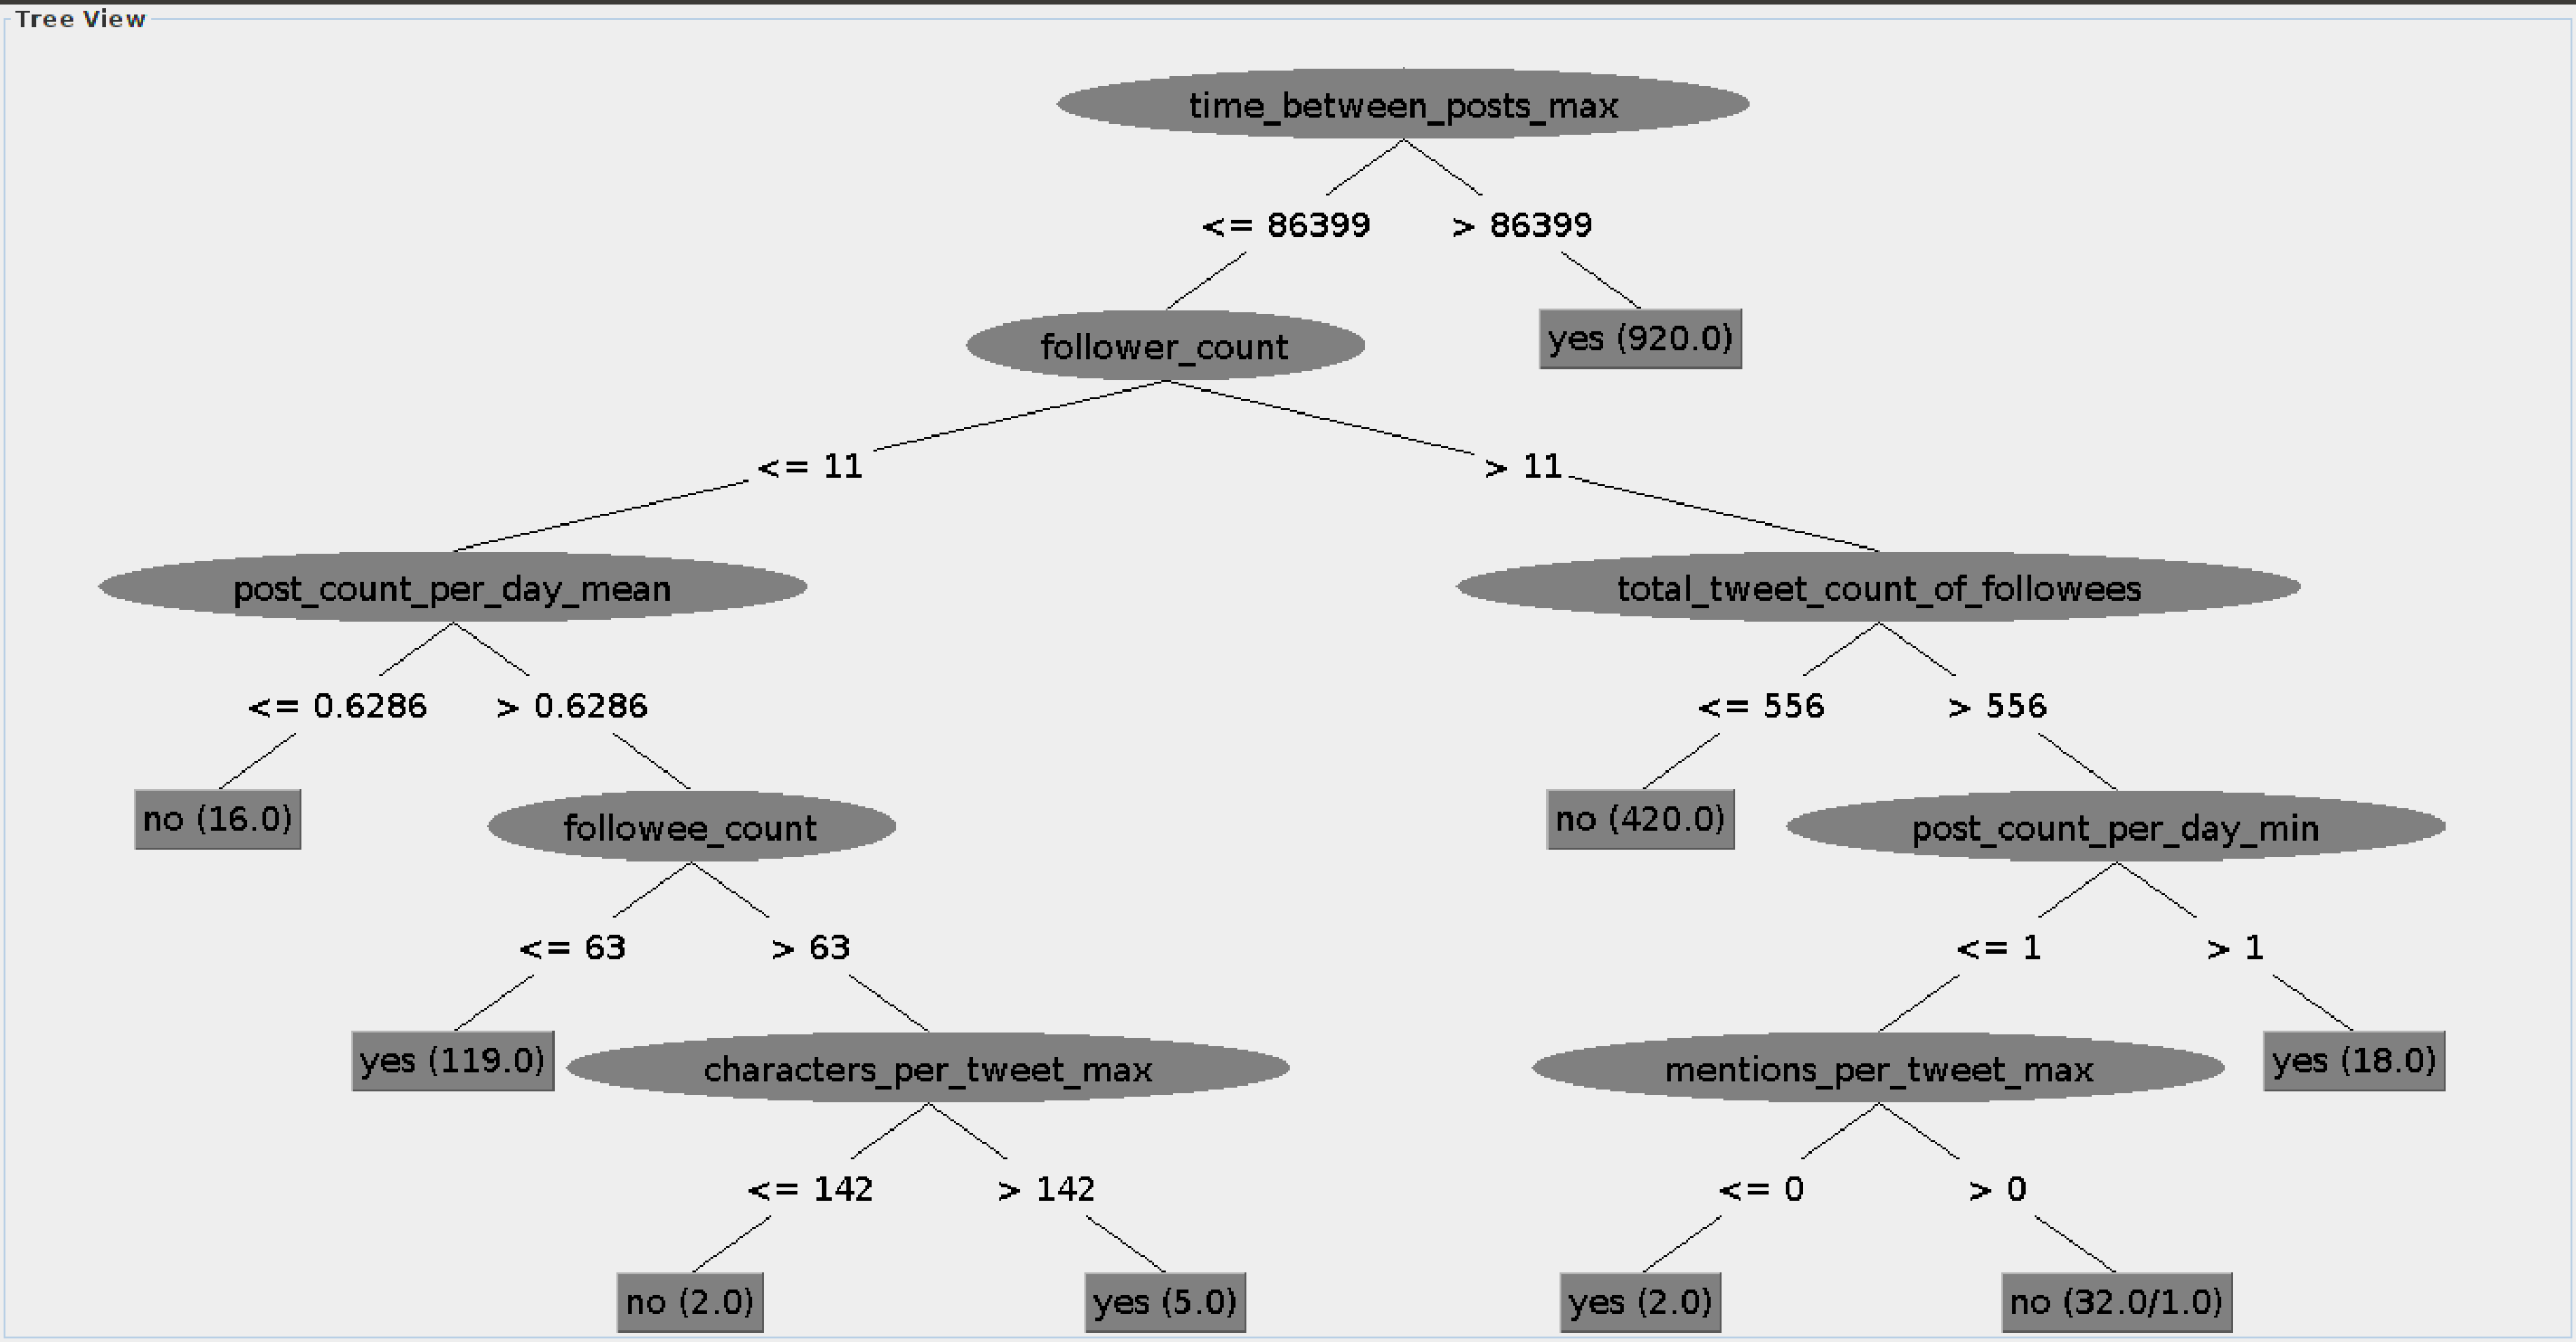
\includegraphics[width=0.95\textwidth,natwidth=610,natheight=642]{classifier.pdf}
\caption{J48 Classifier}
\end{figure}

Figure 3 represents the decision tree used in classification. It is important to validate the decision tree with the data. One of the main attribute as defined by the classifier is the max time between posts. When it is above a certain value, the user always tend to be a spammer. And this tends to be true for 920 cases. Hence, almost 70\% can be classified using this one feature. Also it can be observed that total tweets of friends is a good characteristic feature. It classifies 420 non spammers at just one level. Such attributes which partitions the data clearly are the most important ones. In this regard, important features are,
\newline
\begin{enumerate}
\item maximum time between posts %\\*
\item follower count %\\*
\item mean post count per day %\\*
\item total tweet count of all friends %\\*
\item followee count %\\*
\item minimum post count per day %\\*
\item maximum character per tweet %\\*
\item maximum mentions per tweet %\\*
\end{enumerate}

Hence a reduced feature set would also work as good as the original one. This is proposed due to the huge number of features which could get cumbersome in some cases. 

\section{Conclusion and Future Work}

Due to the importance and indispensability of detecting and preventing Twitter spammers, Twitter corporation as well as many researchers devoted themselves into keep the spammers away from the social network, however, Twitter spammers are evolving to hide from the identification techniques. A continuous understanding of how the spammers evolve through the network is necessary. Since, any feature can be worked around by the spammers, unsupervised learning looks like the way to move forward. Whatever the scheme be, spammers has to tweet to attain their goal.
This creates a separate cluster of people which keeps tweeting to other ordinary user groups that does not follow the cluster. The direction of communication is one directional. This is an idea to identify a group of spammers.

The work we did in this project nailed it where it assumed that the current trends are the most exploited by twitter spammers. But the drawback was that we were not able to get enough data and literally no data on spammers.
Here's an idea to get spammer data to test the classifier. Twitter nowadays are much faster in reacting to spammers and block spammers sometimes within 10 minutes from its creation. So, when data is collected from streaming API, instead of getting just the user obejects, whole feature set can be extracted. This is because, once twitter blocks a person, API access to the person's info will not be available. Now, if the user is blocked at a later time, we can know for sure that the user is a spammer. This can be done going forward. Another thing is, being able to get all features as mentioned in the research work.

\begin{thebibliography}{99}


\bibitem {1}Fabricio Benevenuto, Gabriel Magno, ``Detecting Spammers on Twitter," \emph{Annual Collaboration, Electronic messaging, Anti-
abuse and Spam Conference}, 2010.

\bibitem {2}A. A. Amleshwaram, N. Reddy, ``Cats:
Characterizing automation of twitter spammers" \emph{International Conference on Communication System and Networks}, 2013.

\end{thebibliography}

\newpage
\appendix
\renewcommand\thesection{\appendixname~\Alph{section}}
\renewcommand\theequation{\Alph{section}.\arabic{equation}}
\section{Data collected}
	We consider the following content attributes: \\*
	\newline
fraction of tweets with URLs, \\*
number of hashtags per number of words on each tweet (mean), \\*
number of hashtags per number of words on each tweet (median), \\*
number of hashtags per number of words on each tweet (min), \\*
number of hashtags per number of words on each tweet (max), \\*
number of URLs per number of words on each tweet (mean), \\*
number of URLs per number of words on each tweet (median), \\*
number of URLs per number of words on each tweet (min), \\*
number of URLs per number of words on each tweet (max), \\*
number of characters per tweet (mean), \\*
number of characters per tweet (median), \\*
number of characters per tweet (min), \\*
number of characters per tweet (max), \\*
number of hashtags per tweet (mean), \\*
number of hashtags per tweet (median), \\*
number of hashtags per tweet (min), \\*
number of hashtags per tweet (max), \\*
number of mentions per tweet (mean), \\*
number of mentions per tweet (median),\\*
number of mentions per tweet (min),\\*
number of mentions per tweet (max),\\*
number of numeric characters per tweet (mean),\\*
number of numeric characters per tweet (median),\\*
number of numeric characters per tweet (min),\\*
number of numeric characters per tweet (max),\\*
number of URLs on each tweet (mean),\\*
number of URLs on each tweet (median),\\*
number of URLs on each tweet (min),\\*
number of URLs on each tweet (max),\\*
number of words per tweet (mean),\\*
number of words per tweet (median),\\*
number of words per tweet (min),\\*
number of words per tweet (max),\\*
number of times the tweet has been retweeted (mean),\\*
number of times the tweet has been retweeted (median), \\*
number of times the tweet has been retweeted (min), \\*
number of times the tweet has been retweeted (max).

\newpage
We consider the following user behavior attributes: \\*
\newline
fraction of tweets replied,\\*
number of followees,\\*
number of followers,\\*
number of tweets,\\*
number of followees of a user's followers,\\*
number of times mentioned,\\*
number of times the user was replied,\\*
number of times the user replied,\\*
number of tweets of a user's followees,\\*
time between posts (mean),\\*
time between posts (median),\\*
time between posts  (min),\\*
time between posts (max),\\*
number of posted tweets per day (mean),\\*
number of posted tweets per day (median),\\*
number of posted tweets per day (min),\\*
number of posted tweets per day (max),\\*
number of posted tweets per week (mean),\\*
number of posted tweets per week (median),\\*
number of posted tweets per week (min),\\*
number of posted tweets per week (max).\\*
\end{document}
